% Created 2021-10-26 Tue 18:26
\documentclass[11pt]{article}
\usepackage[utf8]{inputenc}
\usepackage[left=1.2in,right=1.2in]{geometry}
\usepackage[T1]{fontenc}
\usepackage{fixltx2e}
\usepackage{graphicx}
\usepackage{longtable}
\usepackage{float}
\usepackage{subcaption}
%\usepackage{wrapfig}
\usepackage{rotating}
%\usepackage[normalem]{ulem}
\usepackage{amsmath}
\usepackage{textcomp}
%\usepackage{marvosym}
%\usepackage{wasysym}
\usepackage{amssymb}
\usepackage{hyperref}
\tolerance=1000
\author{Mridul Gupta(AIZ218322)}
\date{\today}
\title{COL774 Assignment 3}
\hypersetup{
  pdfkeywords={},
  pdfsubject={},
  pdfcreator={Emacs 25.2.2 (Org mode 8.2.10)}}
\begin{document}

\maketitle
\section{Q1}
\label{sec-1}
\subsection{Q1(a)}
\label{sec-1-1}
\begin{figure}[!ht]
	\subfloat[with one-hot]{%
		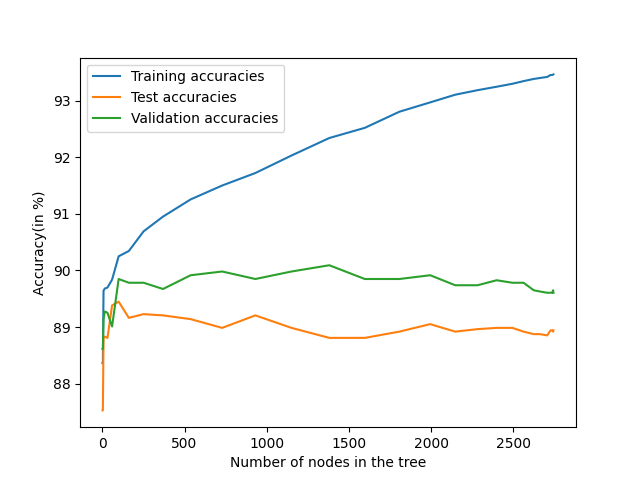
\includegraphics[width=.5\linewidth]{/home/anupam/Desktop/backups/COL774/src/q1/Accuracies_with_onehot.png}
	}
	\subfloat[without one-hot]{%
		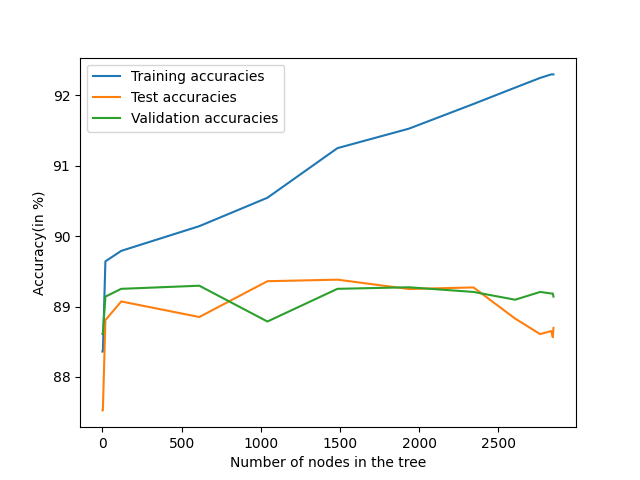
\includegraphics[width=.5\linewidth]{/home/anupam/Desktop/backups/COL774/src/q1/Accuracies_without_onehot.png}
	}
	\caption{Decision Tree Accuracies vs Number of nodes in Tree}
\end{figure}
It seems that the model trained on one-hot encoded data performs
slightly better than the one trained on the not one-hot encoded
data. But what's more important to note here is that the validation
and test accuracy saturate after about a 100 nodes are created and
pretty much oscillate slightly. We can remove these extra nodes and
improve out inference time. I don't know what this will be called, as
the performance on train data improves, but performance on
test/validation doesn't deteriorate. This does not seem to be
overfitting, so no comments can be made about overfitting. Accuracy
was 88.70\(\%\)

\subsection{Q1(b)}
\label{sec-1-2}
Decision tree pruning is performed in bottom-up fashion, the increase
in accuracy is only \(0.2-0.3\%\). Accuracy was \(88.80\%\).
\subsection{Q1(c)}
\label{sec-1-3}
The accuracies obtained are as follows:
\begin{align*}
\text{Train: }&98.11\%\\
\text{Validation: }&90.69\%\\
\text{Test: }&90\%
\end{align*}
The best parameters obtained were \texttt{n\_estimators: 100},
\texttt{max\_features:0.9},\\ \texttt{min\_samples\_split: 10}. The random forest
performs better than pruned decision tree, especially on the training
set. The performance on test set is not very different.
\subsection{Q1(d)}
\label{sec-1-4}
\begin{figure}[!htpb]
	\subfloat[n-estimators]{%
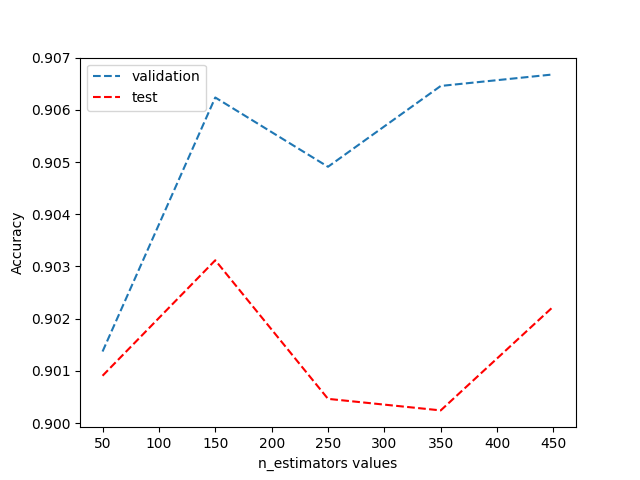
\includegraphics[width=.55\linewidth]{/home/anupam/Desktop/backups/COL774/src/q1/sensitivity_n_estimators.png}
	}
	\subfloat[max-feature]{%
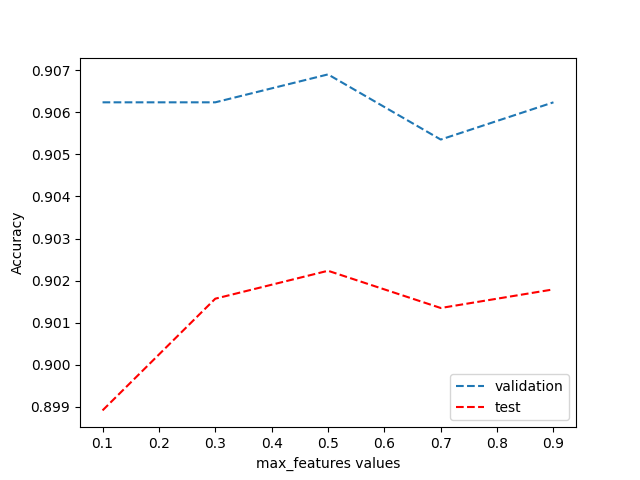
\includegraphics[width=.55\linewidth]{/home/anupam/Desktop/backups/COL774/src/q1/sensitivity_max_features.png}
	}\\
	\begin{center}
	\subfloat[min-samples-split]{%
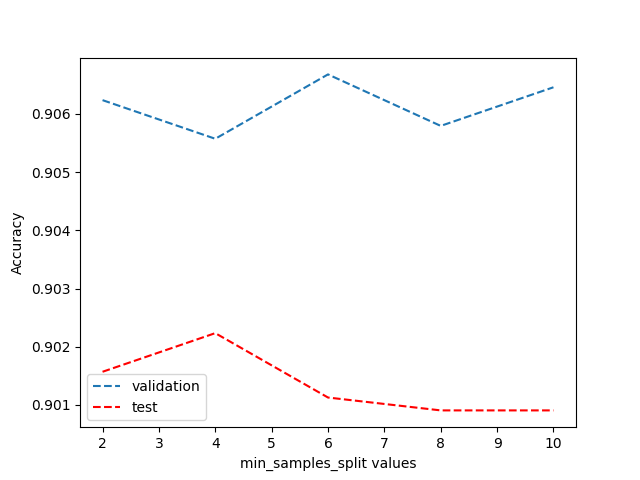
\includegraphics[width=.6\linewidth]{/home/anupam/Desktop/backups/COL774/src/q1/sensitivity_min_samples_split.png}
	}
	\end{center}
	\caption{Sensitivity for parameters}
\end{figure}
It is seen that random forests are most sensitive to n\_estimators as
one would expect, since more models in the ensemble, the better the
estimate as the law of large number suggests (because this is just a
case of averaging out the predictions). Even then, the sensitivity is
not a lot, the algorithm is pretty much stable.

\section{Q2}
\label{sec-2}
\subsection{Q2(a)}
\label{sec-2-1}
I performed one-hot encoding using pandas' \texttt{get\_dummies} function.
\subsection{Q2(b)}
\label{sec-2-2}
For the implementation of the backpropagation algorithm for neural
networks, I follow Goodfellow et al.'s Deep Learning\cite{goodfellow}
(Section 6.5.6 General back-propagation p. 213). I use the tensorflow
api style with reference from codingame.com\cite{codingame}.
\subsection{Q2(c)}
\label{sec-2-3}
\begin{figure}[!ht]
	\subfloat[Accuracy]{%
\includegraphics[width=.5\linewidth]{/home/anupam/Desktop/backups/COL774/src/q2/backup/acc.png}
	}
	\subfloat[Training Time]{%
\includegraphics[width=.5\linewidth]{/home/anupam/Desktop/backups/COL774/src/q2/backup/times.png}
	}
	\caption{Metric vs number of hidden layer nodes Q2(c)}
\end{figure}
\begin{figure}[!ht]
	\subfloat[5]{%
\includegraphics[width=.5\linewidth]{/home/anupam/Desktop/backups/COL774/src/q2/backup/hidden_5.png}
	}
	\subfloat[10]{%
\includegraphics[width=.5\linewidth]{/home/anupam/Desktop/backups/COL774/src/q2/backup/hidden_10.png}
	}\\
	\subfloat[15]{%
\includegraphics[width=.5\linewidth]{/home/anupam/Desktop/backups/COL774/src/q2/backup/hidden_15.png}
	}
	\subfloat[20]{%
\includegraphics[width=.5\linewidth]{/home/anupam/Desktop/backups/COL774/src/q2/backup/hidden_20.png}
	}\\
	\subfloat[25]{%
\includegraphics[width=.5\linewidth]{/home/anupam/Desktop/backups/COL774/src/q2/backup/hidden_25.png}
	}
	\subfloat[100]{%
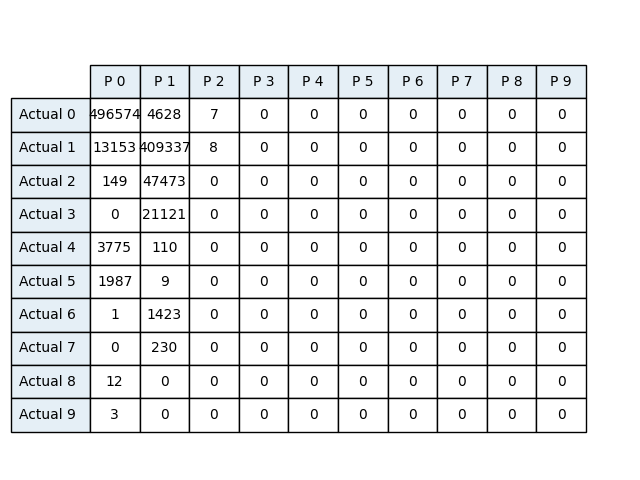
\includegraphics[width=.5\linewidth]{/home/anupam/Desktop/backups/COL774/src/q2/backup/hidden_100.png}
	}
	\caption{Confusion matrix for Q2(c)}
\end{figure}
It is seen that the accuracy and training time both increase as we
increase the number of nodes in the hidden layer of the neural
network. Note, I also train a network with 100 nodes along with the
required \(\{5,10,15,20,25\}\) for this exercise.
For stopping criteria I followed the following intuition: since the
target/label is a one-hot vector for a 10 class classification
problem, it will be a sparse vector with exactly one 1 and the rest
entries being 0. When the network learns that it must output a one hot
vector too, then each incorrect classification will incur an MSE
of 2. Thus, per 100 examples, if the classifier makes one mistake then
the loss function value will be under 0.1. This is what I use for
stopping criteria, that the loss is less than some threshold. Of
course, the sigmoid output is not perfect 0 or 1, thus I try for
various values, and choose the stopping criteria as loss getting lower
than 0.01.
\clearpage
\subsection{Q2(d)}
\label{sec-2-4}
The adaptive learning makes training stable, not necessarily
faster. It is seen that just like the previous case, the training time
and accuracy both go up as the number of nodes is increased. It is
also seen that as the number of nodes go up, the accuracy goes down
because deeper networks do not train well with decreasing learning
rate.
\begin{figure}[!ht]
	\subfloat[Accuracy]{%
\includegraphics[width=.5\linewidth]{/home/anupam/Desktop/backups/COL774/src/q2/backup_adaptive/acc.png}
	}
	\subfloat[Training Time]{%
\includegraphics[width=.5\linewidth]{/home/anupam/Desktop/backups/COL774/src/q2/backup_adaptive/times.png}
	}
	\caption{Metrics vs hidden layer nodes with adaptive learning Q2(d)}
\end{figure}
\begin{figure}[!ht]
	\subfloat[5]{%
\includegraphics[width=.5\linewidth]{/home/anupam/Desktop/backups/COL774/src/q2/backup_adaptive/hidden_5.png}
	}
	\subfloat[10]{%
\includegraphics[width=.5\linewidth]{/home/anupam/Desktop/backups/COL774/src/q2/backup_adaptive/hidden_10.png}
	}\\
	\subfloat[15]{%
\includegraphics[width=.5\linewidth]{/home/anupam/Desktop/backups/COL774/src/q2/backup_adaptive/hidden_15.png}
	}
	\subfloat[20]{%
\includegraphics[width=.5\linewidth]{/home/anupam/Desktop/backups/COL774/src/q2/backup_adaptive/hidden_20.png}
	}\\
	\subfloat[25]{%
\includegraphics[width=.5\linewidth]{/home/anupam/Desktop/backups/COL774/src/q2/backup_adaptive/hidden_25.png}
	}
	\caption{Confusion matrices with adaptive learning for different number of hidden nodes for Q2(d)}
\end{figure}

\clearpage
\subsection{Q2(e)}
\label{sec-2-5}
In this part, the multilayered architecture with \textbf{ReLU}
activation trains to 92.297\(\%\) accuracy within 100 epochs, under 2
minutes. The \textbf{sigmoid} hidden unit architecture however doesn't
converge even after 1400 epochs, and only achieves 77.26\(\%\)
accuracy on test set by then. ReLU performs better than sigmoid in
terms of training speed.
\begin{figure}[!ht]
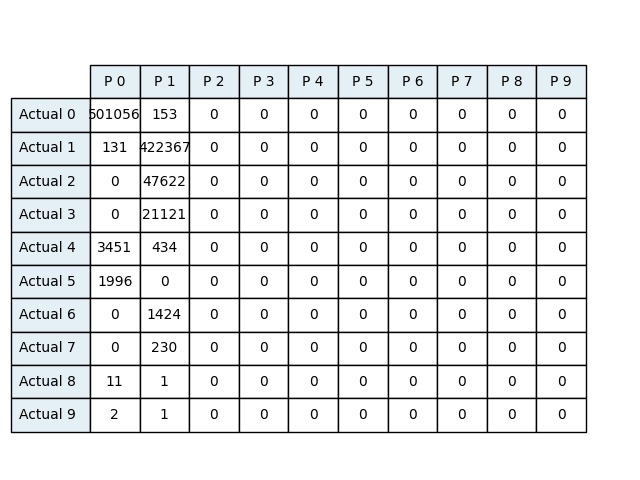
\includegraphics[width=.9\linewidth]{/home/anupam/Desktop/backups/COL774/src/q2/backup_adaptive/hidden_100_100_relu.png}
	\caption{Confusion matrix for Q2(e) with ReLU}
\end{figure}
\begin{figure}[!ht]
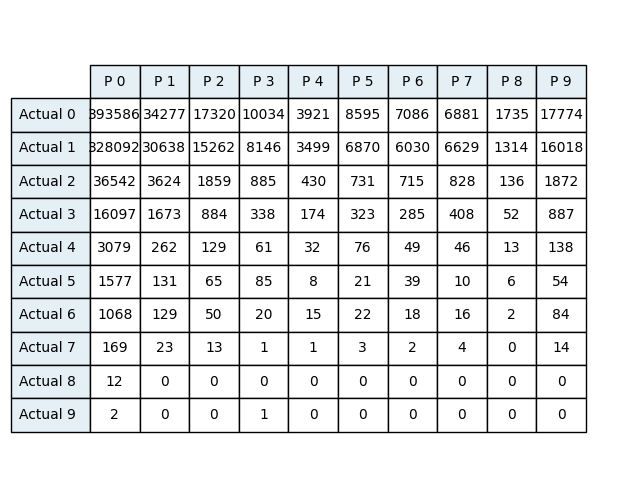
\includegraphics[width=.9\linewidth]{/home/anupam/Desktop/backups/COL774/src/q2/backup_adaptive/hidden_100_100.png}
	\caption{Confusion matrix for Q2(e) with sigmoid}
\end{figure}
\clearpage
\subsection{Q2(f)}
\label{sec-2-6}
The MLPClassifier from sklearn does not work as one would expect. I
initialized the classifier to replicate the training settings and
model architecture exactly as done in Q2(e), yet it doesn't converge
even after 800 epochs, and the maximum accuracy achieved over multiple
trials was under 70\(\%\).
\begin{figure}[!ht]
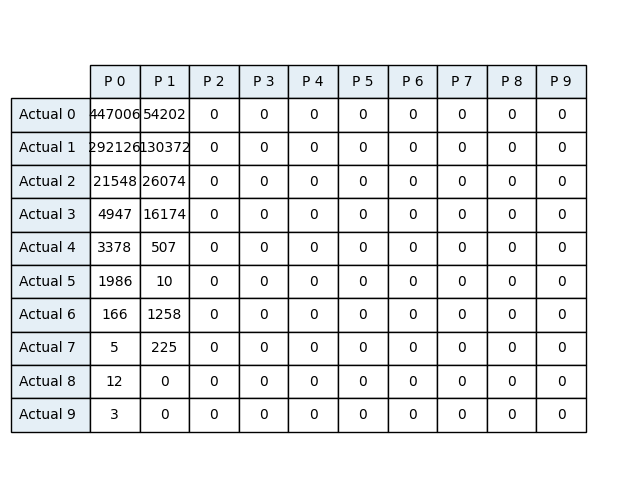
\includegraphics[width=.9\linewidth]{/home/anupam/Desktop/backups/COL774/src/q2/conf_mat_sklearn_relu.png}
	\caption{Confusion matrix for Q2(f) with MLPClassifier}
\end{figure}
\subsection{Q2(g)}
\label{sec-2-7}
I created more samples for classes 6, 7, 8, and 9 by permuting and
undersampled classes 1 and 2 to balance out the training data. The
training completes in under 3 minutes with around \(94\%\)
accuracy. But what is more interesting is that the classifier now
predicts more than just two classes as apparent from the confusion
matrix. Note, I used the two hidden layers with 100 nodes each with
ReLU activation as in Q2(e) for this.
\begin{figure}[!ht]
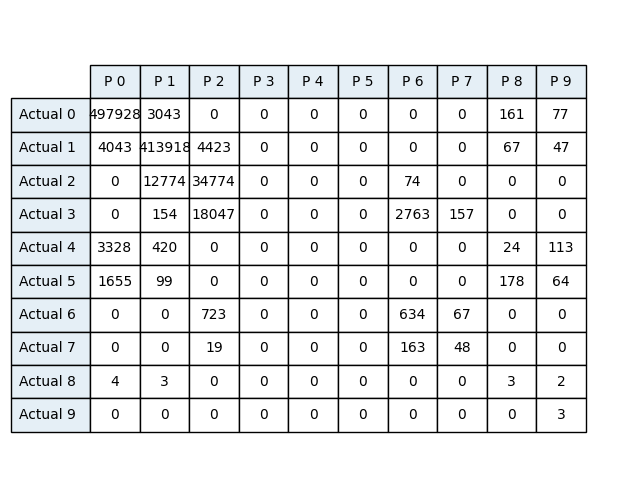
\includegraphics[width=.9\linewidth]{/home/anupam/Desktop/backups/COL774/src/q2/hidden_bal.png}
	\caption{Confusion matrix for Q2(g)}
\end{figure}


\clearpage
\begin{thebibliography}{9}
\bibitem{goodfellow} I. Goodfellow, Y. Bengio and A. Courville, \emph{Deep Learning}, MIT Press, 2016.
\bibitem{codingame} codingame, \lq\lq Deep Learning From Scratch\rq\rq, https://www.codingame.com/playgrounds/9487/deep-learning-from-scratch--theory-and-implementation/computational-graphs, accessed: 2021-10-14
\end{thebibliography}
% Emacs 25.2.2 (Org mode 8.2.10)
\end{document}
